\chapter{Разработка алгоритмов управления БОЭП} \label{ch:ch4}

Объектом исследования является системы автоматического управления (САУ) оптико-электронным прибором (ОЭП) в пространстве по азимуту и углу места в режимах наведения и стабилизации.

Цель работы – является разработка компьютерной имитационных моделей изолированных каналов управления ОЭП, управляемого моментными двигателями по азимуту и углу места и исследование его динамических свойств.
В процессе работы проводились выбор моментных двигателей, синтез алгоритмов управления, разработка компьютерных имитационных моделей изолированных нелинейных каналов управления бортового ОЭП и исследование динамики управления им в режимах наведения и стабилизации.

В результате исследования динамики предложены алгоритмы управления и требования к структуре и элементам изолированных каналов управления, обеспечивающие требования ТЗ, которые будут уточнены при исследовании пространственной задачи управления.

Эффективность управления в режиме наведения достигается применением оптимального управления по быстродействию. 
Все расширяющийся круг военных и гражданских задач, для решения которых широко используются оптико-электронные методы и средства, вызвало интерес к решению научно- технических   проблем, возникающих при решении этих задач [12], [26].

Одна из важных проблем – это влияние динамики и управления на достижение требуемых тактико- технических характеристик бортовых ОЭП и комплексов. Вопросы разработки, моделирования и исследования динамических систем, в том числе бортовых оптико-электронных комплексов, отражены в трудах международных Четаевских конференций по аналитической механике, устойчивости и управлению; в трудах международных симпозиумов по автоматическому управлению и всесоюзных совещаниях по теории инвариантности, в трудах КАИ, а также в журналах: «Оптический журнал», «Гироскопия и навигация», «Оптико-механическая промышленность», «Автоматика и телемеханика», «Авиационная техника», «Вестник КГТУ им. А. Н. Туполева» [4-26]. Разработке алгоритмов и исследованию динамики, и управлению посвящены работы [3 - 29].

На данном этапе разработки выполняемой НИР проведены предварительные расчеты по уяснению решаемых задач и анализу исходных данных, оговоренных техническим заданием (ТЗ), разработке и согласованию
расчетных оптико – механической схем и параметров ОЭП, приводов, датчиков угла САУ с учетом их технических требований и внешних воздействий от носителя.


\section{Технические требования и режимы управления ОЭП} \label{ch:ch4/sect1}

В соответствии с требованиями ТЗ были проанализированы, уточнены, доопределены следующие исходные данные, необходимые для расчета:
\begin{itemize}
	\item Состав системы автоматического управления,
	\item САУ по азимуту,
	\item САУ по углу места,
	\item Датчики углового положения по азимуту и углу места,
	\item Двигатели типа ДБМ (уточняются в процессе разработки) по азимуту и углу места,
	\item Усилительно-преобразовательные блоки каналов управления совместно с микропроцессорными блоками,
	\item Назначение и технические требования.
\end{itemize}
САУ предназначена для наведения оси визирования на заданные угловые координаты относительно строительных осей летательного аппарата (ЛА), параметры движения ЛА.

\newpage
%%%%%%%%%%%%%%%%%%%% Table No: 9 starts here %%%%%%%%%%%%%%%%%%%%

\begin{table}[!h]
	\caption{Технические параметры САУ}%
	\label{tab:SAU_PARAM}% label всегда желательно идти после caption
	\begin{longtable}{|m{5cm}|m{5.5cm}|m{5.5cm}|}
		\hline
		& по азимуту & по углу места \\ 
\hline
Пределы наведения		& $\pm$ 180 град           & (-60 .. +30) град              \\ 
\hline
Максимальная скорость наведения		&600 град/сек            &300 град/сек               \\ 
		\hline
Максимальная среднеквадратическая погрешность наведения и стабилизации		&<30 угловых минут           &<30 угловых минут               \\ 
		\hline
Время наведения на предельный угол		&<0.6 с            & <0.6 с              \\ 
		\hline
Синусоидальные вибрации		& \multicolumn{2}{m{11cm}|}{
	\begin{tabular}[l]{m{11cm}}
		Частота 5-10 Гц, амплитуда перемещения 5 мм\\
		Частота 20-22 Гц, ускорение $25 \textit{м/с}^2$\\
		Частота 35,4-50 Гц, амплитуда перемещения 0.5 мм\\
		Частота 50-500 Гц, ускорение $25 \textit{м/с}^2$
	\end{tabular}

}      \\ 
		\hline
Требования к САУ при внешних воздействиях		& \multicolumn{2}{m{11cm}|}{\begin{tabular}[l]{m{11cm}}
		максимальной скорости движения носителя – 56 м/с (200км/час)\\
		максимальный крен ЛА $\leq 15^0$\\
		угловая скорость носителя $\omega_y=12$ град/c\\
		минимальная высота полета носителя – 1500 м\\
		максимальная скорость движения ОН – 500 м/с	
\end{tabular}}      \\ 
		\hline
Гармонические возмущения, идущие от ЛА по азимуту и углу места		& \multicolumn{2}{m{11cm}|}{\begin{tabular}[l]{m{11cm}}
		Частота 0.16 Гц, амплитуда колебаний 12 град.\\
		Частота 1 Гц, амплитуда колебаний 1- 2 град.
\end{tabular}}      \\ 
		\hline
Требования к САУ при воздействиях ускорений в условиях движения носителя		& \multicolumn{2}{m{11cm}|}{$4.8 \textit{м/с}^2$}      \\ 
		\hline
	\end{longtable}
\end{table}

%%%%%%%%%%%%%%%%%%%% Table No: 9 ends here %%%%%%%%%%%%%%%%%%%%

Геометрия масс тел вращения объекта управления (ОУ) по двум осям управления опредставлена в таблице \ref{tab:SAU_PARAM} и рисунокe \ref{fig:41}.

%%%%%%%%%%%%%%%%%%%% Figure/Image No: 30 starts here %%%%%%%%%%%%%%%%%%%%

\begin{figure}[!ht]
	\centering
	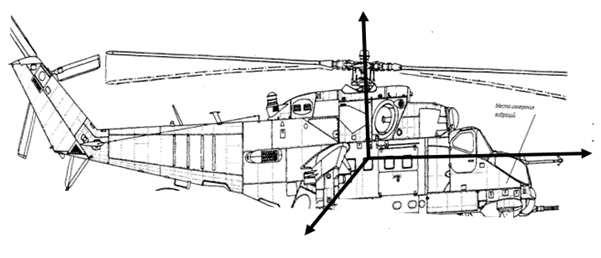
\includegraphics[width=0.8\linewidth]{img-25} 
	\caption{Обозначение строительных осей ЛА}
	\label{fig:41}
\end{figure}

%%%%%%%%%%%%%%%%%%%% Figure/Image No: 30 Ends here %%%%%%%%%%%%%%%%%%%%

В отчете приведены синтез алгоритмов управления, разработка компьютерных моделей и исследование динамики изолированных каналов управления САУ с учетом частоты ШИМ и насыщения усилителей мощности, дискретизации датчиков угла.


\section{Обоснование выбора приводов} \label{ch:ch4/sect2}

\section{Уравнения движения изолированных каналов управления} \label{ch:ch4/sect3}


\subsection{Уравнения движения привода по азимуту} \label{subsec:ch4/sect3/sub1}


\subsection{Уравнения движения привода по углу места} \label{subsec:ch4/sect3/sub2}

\section{Синтез алгоритмов управления ОЭП} \label{ch:ch4/sect4-}

В соответствии с ТЗ управление ОЭП проводится в двух режимах:
наведения ОЭП на объект наблюдения (ОН) и стабилизации оптической оси относительно направления на ОН. 

Синтез алгоритмов управления проводился частотным методом [27] для каждого из режимов. На основе полученных законов управления разработаны компьютерные модели (КМ) линейной и нелинейной САУ в среде Simulink MatLAB и проведены исследования динамики САУ с помощью КМ в режимах наведения и стабилизации при действии возмущений, оговоренных в ТЗ.

Структурная схема САУ изолированного канала показана на рисунке \ref{fig:structured_SAU}.

\begin{figure}[ht]
	\centering
	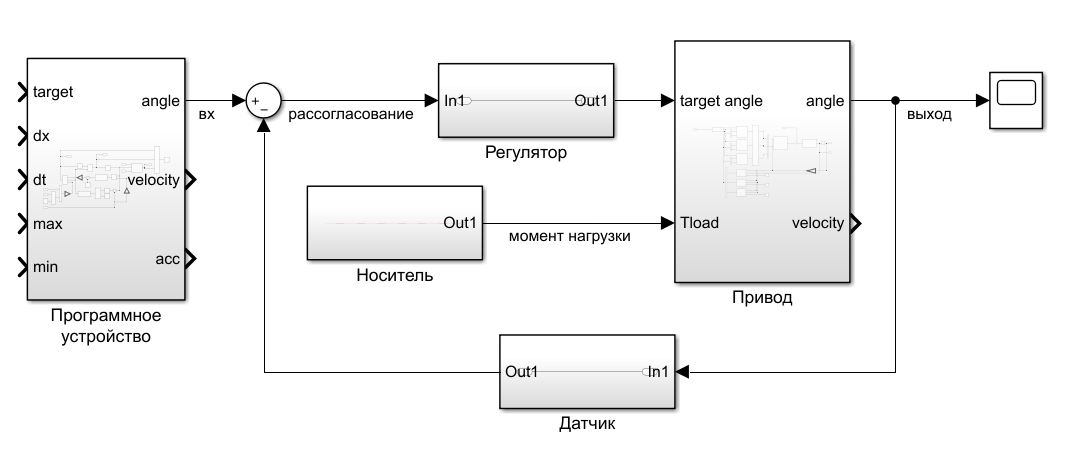
\includegraphics[width=0.8\linewidth]{structured_SAU}
	\caption{Структурная схема САУ}
	\label{fig:structured_SAU}
\end{figure}

Программное устройство определяет режим работы и задает целевое значение положения ротора канала, регулятор обеспечивает оптимальную работу привода, привод - объект управления , 
датчик угла измеряет положение ротора, "носитель" определяет внешние возмущающие факторы влияющие на систему.


\section{Синтез алгоритмов программного устройства} \label{ch:ch4/sect2+}

\subsection{Режим наведения} \label{subsec:ch4/sect2/sub1}

Режим наведения должен осуществляться в пределах заданых углов относительно ЛА ($\varDelta\alpha$) за время ($\varDelta t$). Для решения этой задачи управления рассмотрим оптимальное управление по быстродействию [3, 27].

Задача устройства состоит в том чтобы выдать оптимальную траекторию движения основываясь на следующих условиях:
\begin{enumerate}
	\item средняя скорость разворота должна удовлетворять требованиям ТУ: 
	$\frac{\varDelta\alpha}{\varDelta t}$
	\item скорость движения в начальный и конечным момент должна быть равна 0
	\item программный угол не должен выходить за заданые пределы
\end{enumerate}

Построим программное устройство (ПУ), предназначенное для выдачи требуемой программной траектории движения оптической оси на основе решения уравнений:
\begin{equation}
\label{eq:p4:2+.1}
\begin{alignedat}{2}
\varDelta\alpha = \dfrac{\ddot{\alpha}{\varDelta t}^2}{4}
\end{alignedat}
\end{equation}

Схема моделирования ПУ приведена на рисунке \ref{fig:model_control}. Фрагмент решения уравнений (\ref{eq:p4:2+.1}) приведен далее (рисунок \ref{fig:model_control_graph}).

\begin{figure}[ht]
	\centering
	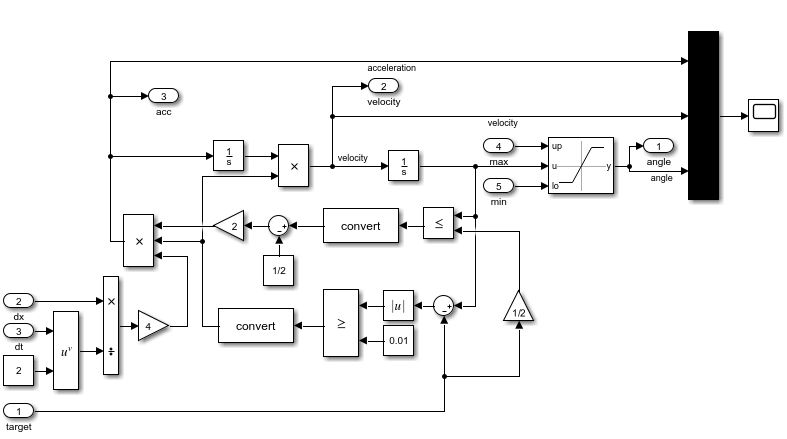
\includegraphics[width=1.0\linewidth]{model_control} 
	\caption{Схема моделирования программного устройства}
	\label{fig:model_control}
\end{figure}



\begin{figure}
	\centering
	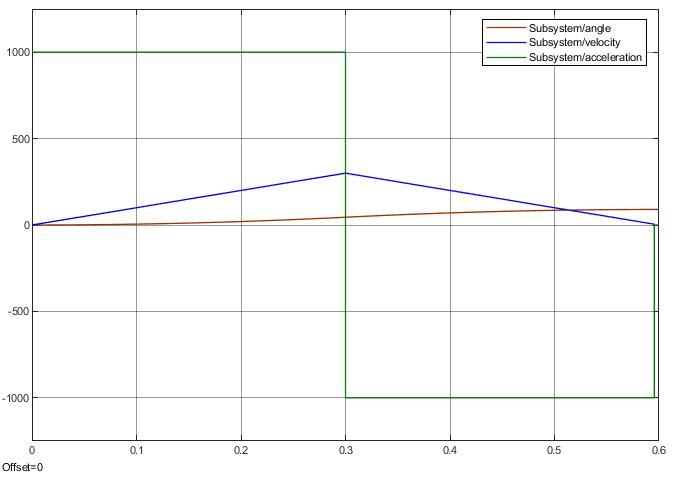
\includegraphics[width=1.0\linewidth]{model_control_graph}
	\caption{График ускорения, скорости и координаты программного движения}
	\label{fig:model_control_graph}
\end{figure}


\section{Синтез алгоритмов управления ОЭП, моделирование и исследование динамики САУ по азимуту в режиме наведения} \label{ch:ch4/sect4}


\subsection{Синтез и исследование линейной системы управления} \label{subsec:ch4/sect4/sub1}


\subsection{Синтез, моделирование и исследование динамики нелинейной САУ} \label{subsec:ch4/sect4/sub2}


\subsection{Синтез цифровых САУ } \label{subsec:ch4/sect4/sub3}


\subsection{Моделирование и исследование динамики ЦСАУ} \label{subsec:ch4/sect4/sub4}


\section{Синтез алгоритмов управления ОЭП, моделирование и исследование динамики САУ  по углу места  в режиме наведения} \label{ch:ch4/sect5}


\subsection{Синтез и исследование линейной САУ} \label{subsec:ch4/sect5/sub1}


\subsection{Синтез цифровых САУ } \label{subsec:ch4/sect5/sub2}


\subsection{Моделирование и исследование динамики ЦСАУ} \label{subsec:ch4/sect5/sub3}



\section{Моделирование и исследование динамики изолированных каналов управления ОЭП в режиме стабилизации} \label{ch:ch4/sect6}


\subsection{Моделирование и исследование динамики нелинейной САУ по курсу} \label{subsec:ch4/sect6/sub1}


\subsection{Моделирование и исследование динамики нелинейной САУ по углу места} \label{subsec:ch4/sect6/sub2}


\section{Анализ результатов исследований и определение требований к элементам САУ} \label{ch:ch4/sect7}


\section{Выводы по главе} \label{ch:ch4/sect8}



Некоторый текст.

\clearpage